\documentclass{svproc}

\usepackage{url}
\usepackage{amsmath}
\usepackage{amssymb}
\usepackage{soul}
\usepackage{graphicx}
\usepackage{seqsplit}
\usepackage{tikz}
\usepackage[ruled,vlined,linesnumbered]{algorithm2e}
\usepackage[colorlinks=true, linkcolor=blue, citecolor=blue, urlcolor=blue]{hyperref}

\SetKwProg{Let}{let}{be:}{}
\usetikzlibrary{arrows, decorations.pathmorphing, decorations.markings, shapes.geometric, calc, positioning}

\tikzset{
    node0/.style={circle, draw, fill=white, inner sep=0pt, minimum size=1.5mm},
    node1/.style={circle, draw, fill=black, inner sep=0pt, minimum size=1.5mm},
    reoEdge/.style={->, >=latex, thin},
    reoSpout/.style={<->, >=latex, thin},
    reoLossy/.style={->, >=latex, thin, dashed},
    reoWavy/.style={->, >=latex, thin, decorate, decoration={zigzag, amplitude=1mm, segment length=1.5mm, post length=1.5mm, pre length=1.5mm}},
}

% A. 基础连线类 (Sync, Lossy, Filter)  参数: #1=样式(可选), #2=起点, #3=终点, #4=标签文字(可选)
\newcommand{\drawLink}[4][reoEdge]{
    \draw[#1] (#2) -- node[above, font=\scriptsize] {#4} (#3);
}

% B. FIFO 类 (中间带方框)  参数: #1=起点, #2=终点, #3=方框内文字, #4=额外样式(可选,如 dashed)
\newcommand{\drawFIFO}[4][]{
    \draw[reoEdge, #1] (#2) -- node[midway, sloped, allow upside down, draw, fill=white, rectangle, minimum width = 6mm, minimum height = 2mm, inner sep=1pt, font=\tiny] {#4} (#3);
}

% C. Drain 类 (两头向中间汇聚)  参数: #1=起点1, #2=起点2, #3=汇聚点/符号位置(通常是这两个点的中点), #4=中心符号(如 ||)
\newcommand{\drawDrain}[5]{
    % 计算中点
    \coordinate (mid1) at ($(#1)!0.4!(#2)$);
    \coordinate (mid) at ($(#1)!0.5!(#2)$);
    \coordinate (mid2) at ($(#1)!0.6!(#2)$);
    % 画两段箭头指向中点
    \draw[->, >=latex, thin] (#1) -- (mid1);
    \draw[thin] (mid1) -- (mid);
    \draw[thin] (mid) -- (mid2);
    \draw[->, >=latex, thin] (#2) -- (mid2);
    % 画中心符号
    \node at (mid) [font=\tiny, inner sep=1pt] {#3};
    \node at (mid1) [font=\tiny, inner sep=1pt] {#4};
    \node at (mid2) [font=\tiny, inner sep=1pt] {#5};
    % 实际上 Drain 并没有显式的 Sink 节点,这里 #3 只是为了兼容位置逻辑,或者如果不画节点只画线
}

% D. Spout 类 (一点分发给两点)  参数: #1=源点, #2=终点1, #3=终点2, #4=线样式
\newcommand{\drawSpout}[5]{
    % 计算中点
    \coordinate (mid1) at ($(#1)!0.4!(#2)$);
    \coordinate (mid) at ($(#1)!0.5!(#2)$);
    \coordinate (mid2) at ($(#1)!0.6!(#2)$);
    % 画两段箭头指向中点
    \draw[->, >=latex, thin] (mid1) -- (#1);
    \draw[thin] (mid1) -- (mid);
    \draw[thin] (mid) -- (mid2);
    \draw[->, >=latex, thin] (mid2) -- (#2);
    % 画中心符号
    \node at (mid) [font=\tiny, inner sep=1pt] {#3};
    \node at (mid1) [font=\tiny, inner sep=1pt] {#4};
    \node at (mid2) [font=\tiny, inner sep=1pt] {#5};
    % 实际上 Drain 并没有显式的 Sink 节点,这里 #3 只是为了兼容位置逻辑,或者如果不画节点只画线
}

% E. Timer 类 (中间带圆角框)  参数: #1=起点, #2=终点, #3=延迟时间 t
\newcommand{\drawTimer}[3]{
    \draw[reoEdge] (#1) -- node[draw, fill=white, rectangle, rounded corners=2pt, minimum size=3.5mm, inner sep=1pt, font=\tiny] (timerbox) {#3} (#2);
}

% F. 复杂 Timer 类 (带控制端口 OFF/RESET/EXPIRE)  参数: #1=起点, #2=终点, #3=延迟时间 t, #4=控制类型(OFF/RST/EXP), #5=控制节点位置(above/below)
\newcommand{\drawComplexTimer}[5]{
    % 先画基础 Timer
    \draw[reoEdge] (#1) -- node[draw, fill=white, rectangle, rounded corners=2pt, minimum size=3.5mm, inner sep=1pt, font=\tiny] (timerbox) {#3} (#2);
    % 画控制端口
    \node (ctrl) [#5=0.5cm of timerbox, font=\tiny] {#4};
    \draw[->, >=latex, dashed] (ctrl) -- (timerbox);
}


% --- 1. Basic Channels ---
\newcommand{\chanSync}[2]{\drawLink{#1}{#2}{}}
\newcommand{\chanLossySync}[2]{\drawLink[reoLossy]{#1}{#2}{}}
\newcommand{\chanSyncDrain}[2]{\drawDrain{#1}{#2}{}{}{}} % 空心汇聚
\newcommand{\chanAsynDrain}[2]{\drawDrain{#1}{#2}{$||$}{}{}} % 带竖线汇聚
% --- 2. FIFO Variants ---
\newcommand{\chanFifoOne}[2]{\drawFIFO{#1}{#2}{}}          % Buffer size 1
\newcommand{\chanFifoN}[3]{\drawFIFO{#1}{#2}{$N=#3$}}      % Buffer size n
\newcommand{\chanFifoOneE}[3]{\drawFIFO{#1}{#2}{$#3$}}     % Initialized with e
\newcommand{\chanFifoNE}[4]{\drawFIFO{#1}{#2}{$#3$}}    % Initialized e with size n
% --- 3. Filter & Producer ---
\newcommand{\chanFilterP}[3]{\drawLink[reoWavy]{#1}{#2}{$P(#3)$}} 
\newcommand{\chanProducerP}[3]{\drawLink{#1}{#2}{Prod: $#3$}} 
% --- 4. Spouts ---
\newcommand{\chanSyncSpout}[2]{\drawSpout{#1}{#2}{}{}{}}
\newcommand{\chanAsynSpout}[2]{\drawSpout{#1}{#2}{$||$}{}{}}
% --- 5. Probabilistic/Faulty ---
\newcommand{\chanCptSync}[3]{\drawLink{#1}{#2}{$p=#3$}}       % Corrupting Sync
\newcommand{\chanRdmSync}[3]{\drawLink{#1}{#2}{#3}}         % Random Sync
\newcommand{\chanProbLossy}[3]{\drawLink[reoLossy]{#1}{#2}{$p=#3$}} % Probabilistic Lossy
\newcommand{\chanFtyFifoOne}[3]{\drawFIFO{#1}{#2}{Fty:$#3$}} % Faulty FIFO
\newcommand{\chanLossyFifoOne}[3]{\drawFIFO[dashed]{#1}{#2}{Lossy:$#3$}} % Lossy FIFO
% --- 6. Timers ---
\newcommand{\chanTimert}[3]{\drawTimer{#1}{#2}{#3}}
\newcommand{\chanOFFTimert}[3]{\drawComplexTimer{#1}{#2}{#3}{OFF}{above}}
\newcommand{\chanRSTTimert}[3]{\drawComplexTimer{#1}{#2}{#3}{RST}{above}}
\newcommand{\chanEXPTimert}[3]{\drawComplexTimer{#1}{#2}{#3}{EXP}{above}}

\bibliographystyle{splncs03}
\def\UrlFont{\rmfamily}

\begin{document}

\title{Connectors as designs: Refinement and test case generation using Z3}
\titlerunning{Connectors as designs: Refinement and test case generation using Z3}
\author{Sihan Wu\inst{1} \and Xueyi Tan\inst{2}}
\authorrunning{S. Wu and X. Tan}
\tocauthor{Wu, Tan}
\institute{Yuanpei College, Peking University, No.5 Yiheyuan Road, Haidian District, Beijing 100871, China,\\
\email{2300017743@stu.pku.edu.cn},
\and
School of Mathematical Sciences, Peking University, No.5 Yiheyuan Road, Haidian District, Beijing 100871, China,\\
\email{2300010816@stu.pku.edu.cn}}

\maketitle

\begin{abstract}
Reo is a channel-based exogenous coordination language for structuring interactions in distributed systems. This paper proposes a unified framework for modeling, refinement verification, and fault-based test case generation of Reo connectors based on Unifying Theories of Programming (UTP) and the SMT solver Z3. Reo connectors, including basic, timed, and probabilistic ones, are modeled as UTP designs with explicit separation of preconditions and postconditions, making connector causality precise. Refinement is defined via predicate implication in UTP and automatically checked using Z3, which also generates fault-based test cases by searching for bounded counterexamples. To support scalable construction of complex connectors, we introduce \texttt{\seqsplit{automerger}} and \texttt{\seqsplit{multi-merger}} extensions. Experimental results show that the framework effectively supports connector modeling, automated refinement checking, and test case generation.
\keywords{Connector, UTP, Z3, Refinement, Test Case Generation}
\end{abstract}

\section{Introduction}
With the rapid growth of service-oriented computing and distributed systems, the coordination of heterogeneous components has become a fundamental challenge. Conventional ad hoc “glue code” for component interaction lacks a rigorous semantic foundation, often resulting in ambiguous designs and error-prone implementations. Reo, a channel-based exogenous coordination language, addresses this problem by supporting the compositional construction of connectors from primitive channels such as synchronous and FIFO channels, thereby separating coordination concerns from component logic and promoting loose coupling and reusability.\par
The correctness of Reo connectors is crucial to the reliability of distributed systems and calls for formal verification techniques. Existing semantic and verification approaches, however, exhibit notable limitations. In particular, some semantic models do not make the causal relationship between inputs and outputs explicit, while automata-based approaches suffer from scalability issues when handling unbounded data domains or timed and probabilistic behaviors. Moreover, test case generation for Reo connectors remains insufficiently integrated with formal semantic models and automated verification tools.\par
Unifying Theories of Programming (UTP) offers a uniform relational framework for modeling and reasoning about programs and specifications via pre/post-condition designs. Prior work has demonstrated that Reo connectors can be interpreted as UTP designs, enabling formal reasoning about equivalence and refinement, and has further extended this approach to timed and probabilistic connectors. Nevertheless, these approaches largely rely on interactive theorem proving, which limits automation and does not readily provide counterexamples or systematic test cases for invalid refinements.\par
SMT solvers, such as Z3, have shown strong capabilities in automated constraint solving and bounded verification. While recent work has applied Z3 to refinement checking of Reo connectors, support for fault-based test case generation and scalable construction of complex connectors remains limited.\par
To overcome these limitations, this paper presents a unified UTP- and Z3-based framework for the formal modeling, refinement verification, and fault-based test case generation of Reo connectors. Our main contributions are:
\begin{itemize}
    \item modeling basic, timed, and probabilistic Reo connectors in Z3;
    \item automated refinement/equivalence checking using Z3, including fault-based test case generation approach for detecting common connector design errors;
    \item automated support for connector construction via an automerger algorithm and a multi-merger extension.
\end{itemize}
The remainder of the paper is organized as follows. Section \ref{sec:preliminaries} introduces Reo, UTP designs, and Z3. Section \ref{sec:utp-modeling} presents the UTP-based modeling of connectors. Section \ref{sec:z3-refinement} describes Z3-based refinement checking, test case generation, and implementation details. Section \ref{sec:conclusion} concludes the paper and outlines future work.


\section{Preliminaries}
\label{sec:preliminaries}
\subsection{The coordination language Reo}
Reo is a channel-based exogenous coordination language in which complex coordinators, called connectors, are compositionally constructed from simpler ones \cite{Reo}. Exogenous coordination enforces a local interpretation of inter-component communication as pure I/O operations, enabling anonymous interaction through the exchange of untargeted data.\par
In Reo, complex connectors are formed as networks of primitive connectors, called \textit{channels}, with well-defined behavior (e.g., synchronous and FIFO channels). A connector specifies communication, synchronization, and data-flow protocols independently of component logic. Each channel has two \textit{channel ends}, classified as \textit{source} or \textit{sink} ends, which respectively accept and dispense data. Channel ends may be of the same or different types, and Reo imposes no restriction on channel behavior, allowing heterogeneous channel types to coexist within a single connector. Each channel end is connected to at most one component instance at a time.\par
Complex connectors are constructed using the \textit{join} and \textit{hiding} operations. Channels are joined at nodes, each consisting of a set of coincident channel ends that are partitioned into source ends Src($A$) and sink ends Snk($A$). Depending on their incident channel ends, nodes are classified as \textit{source}, \textit{sink}, or \textit{mixed} nodes. The hiding operation abstracts away internal nodes, making them unobservable from outside the connector. A connector is graphically represented as a \textit{Reo circuit}, i.e., a finite graph whose nodes are labeled with disjoint, non-empty sets of channel ends and whose edges represent channels. The observable behavior of a Reo circuit is defined by the data-flow at its source and sink nodes.

\subsection{The UTP observational model}
Specification and unification are recurring phases in scientific inquiry. Specification focuses on narrowly defined phenomena and the laws governing them, while unification seeks general theories that account for a broader range of observations. Such unifying theories complement, rather than replace, the individual theories they relate. In computer science, Hoare and He introduced this unifying perspective through the Unifying Theories of Programming (UTP) \cite{hoare1997unified}.\par
Our theory of Reo connectors is motivated by this unification principle. In this section, we briefly introduce the theory of UTP designs and the observational model used for Reo connectors. Further details on UTP can be found in \cite{hoare1997unified}.

\subsubsection{A theory of designs}
A UTP theory is defined by a collection of relations together with three components: an alphabet, a signature, and a set of healthiness conditions.\par
A direct and obvious way to represent the observable behavior of a connector is to model it as a relation on its inputs and outputs. Because the inputs/outputs take place through the nodes of the connector, sequences of data items that pass through a node together with the moments in time that the data items are observed emerge as the key building blocks for describing connector behavior.\par
In our semantic model, we use two auxiliary Boolean variables \textit{ok} and \textit{ok’} to analyze explicitly the phenomena of communication initialization and termination. The variable \textit{ok} indicates successful initialization and the start of communication; when \textit{ok} is \textbf{false}, no observation is possible. The variable \textit{ok’} represents termination or the attainment of a stable intermediate state; divergence is indicated when \textit{ok’} is \textbf{false}. The observational semantics for a Reo connector is described by a design, i.e., a relation expressed as $P\vdash Q$, where $P$ specifies constraints on observations at the source nodes and $Q$ specifies the required conditions on observations at the sink nodes. Such a design $P\vdash Q$ is formally defined as follows:
\begin{definition}
    A design is a pair of predicates $P\vdash Q$, where neither predicate contains \textit{ok} or \textit{ok'}, and $P$ has only unprimed variables. It has the following meaning:$$P\vdash Q=_{df}(ok\land P\Rightarrow ok'\land Q)$$
    \label{def:1}
\end{definition}
The separation of condition on inputs from condition on outputs in our model allows us to write a specification that has a more generous precondition than simply the domain of a relation used as a specification. We are allowed to assume that the condition on inputs holds, and we have to satisfy the condition on its outputs. Moreover, we can rely on the behavior of a connector having been started, but we must ensure that it terminates. If the condition on inputs does not hold, or the connector does not start its behavior, we are not committed to establish the condition on the outputs nor even to make the connector behavior terminate.\par
In UTP, we have the well-known property for refinement, which is established by the following definition:
\begin{definition}
    $[(P_1\vdash Q_1)\sqsubseteq(P_2\vdash Q_2)]$ \textbf{iff} $[P_1\Rightarrow P_2]\land[P_1\land Q_2\Rightarrow Q_1]$
\end{definition}
Furthermore, there are a family of operators on designs, such as conditional choice, sequential composition, iteration, etc., and a lot of algebraic laws being satisfied by these operators. More detailed discussion on designs can be found in \cite{hoare1997unified}.
Finally, iteration is expressed by means of recursive definitions. A recursively defined design has as its body a function on designs; as such, it can be seen as a (monotonic) function on pre/post-condition pairs $(X, Y)$, and iteration is defined as the least fixed point of the monotonic function.\par
The theory of designs can be taken as a tool for representing specifications, programs, and, as in the following sections, connectors.

\subsubsection{Observational model for connectors}
Connectors describe the coordination among components/services. We use $in_\textbf{R}$ and $out_\textbf{R}$ to denote what happens on the source nodes and the sink nodes of a connector \textbf{R}, respectively, instead of using unprimed variables for initial observations (inputs) and primed variables for subsequent ones (outputs) as in \cite{hoare1997unified}.\par
For an arbitrary connector \textbf{R}, the relevant observations come in pairs, with one observation on the source nodes of \textbf{R}, and one observation on the sink nodes of \textbf{R}. For every node $N$, the corresponding observation on $N$ is given by a (finite or infinite) timed data sequence, which is defined as follows:\par
Let $D$ be an arbitrary set, the elements of which are called data elements. The set $DS$ of data sequences is defined as$$DS=D^*$$
i.e., the set of all sequences $\alpha=(\alpha(0),\alpha(1),\alpha(2),\ldots)$ over $D$. Let $\mathbb{R}^*_+$ be the set of non-negative real numbers, which in the present context can be used to represent time moments.\footnote{Here we use the continuous time model for connectors since it is expressive and closer to the nature of time in the real world.} For a sequence $s$, we use $|s|$ to denote the length of $s$, and if $s$ is an infinite sequence, then $|s|=\infty$. Let $\mathbb{R}^*_+$ be the set of sequences $a=(a(0),a(1),a(2),\ldots)$ over $\mathbb{R}_+$, and for all $a=(a(0),a(1),a(2),\ldots)$ and $b=(b(0),b(1),b(2),\ldots)$ in $\mathbb{R}^*_+$, if $|a|=|b|$, then
\[
\begin{split}
    a<b&\text{\qquad iff\qquad}\forall 0\leq n<|a|.a(n)<b(n)\\
    a\leq b&\text{\qquad iff\qquad}\forall 0\leq n<|a|.a(n)\leq b(n)
\end{split}
\]
For a sequence $a=(a(0),a(1),a(2),\ldots)\in\mathbb{R}^*_+$, and $t\in\mathbb{R}_+$, $a[+t]$ is a sequence defined as follows:
$$a[+t]=(a(0)+t,a(1)+t,a(2)+t,\ldots)$$
Furthermore, the element $a(n)$ in a sequence $a=(a(0),a(1),a(2),\ldots)$ can also be expressed in terms of derivatives $a(n)=a^{(n)}(0)$, where $a^{(n)}$ is defined by 
$$a^{(0)}=a,a^{(1)}=(a(1),a(2),\ldots),a^{(k+1)}=(a^{(k)})^{(1)}$$
The set $TS$ of time sequences is defined as
\[
\begin{split}
    TS=\{a\in\mathbb{R}^*_+\mid&(\forall 0\leq n<|a|.a(n)<a(n+1))\\
    &\land(|a|=\infty\Rightarrow\forall t\in\mathbb{R}_+^*.\exists k\in\mathbb{N}.a(k)>t)\}
\end{split}
\]
Thus, a time sequence $a\in TS$ consists of increasing and diverging time moments $a(0)<a(1)<a(2)<\cdots$.\par
For a sequence $a$, the two operators $a^R$ and $\overrightarrow{a}$ denote the reverse and the tail of $a$, respectively, defined as:
\[
\begin{split}
    a^R&=\begin{cases}
        ()&\text{if }a=()\\
        (a')^{R^{\smallfrown}} (a(0))&\text{if }a=(a(0))^{\smallfrown} a'
    \end{cases}\\
    \overrightarrow{a}&=\begin{cases}
        ()&\text{if }a=()\\
        a'&\text{if }a=(a(0))^{\smallfrown} a'
    \end{cases}
\end{split}
\]
where $^{\smallfrown}$ is the concatenation operator on sequences. The concatenation of two sequences produces a new sequence that
starts with the first sequence followed by the second sequence.\par
The set $TDS$ of timed data sequences is defined as $TDS\subseteq DS\times TS$ of pairs $\langle\alpha,a\rangle$ consisting of a data sequence $\alpha$ and a time sequence $a$ with $|\alpha| = |a|$. Similar to the discussion in \cite{arbab2002coinductive}, timed data sequences can be alternatively and equivalently defined as (a subset of) $(D\times \mathbb{R}_+)^*$ because of the existence of the isomorphism
$$\langle\alpha,a\rangle\mapsto(\langle\alpha(0),a(0)\rangle,\langle\alpha(1),a(1)\rangle,\langle\alpha(2),a(2)\rangle,\ldots)$$
The occurrence (i.e., taking or writing) of a data item at some node of a connector is modeled by an element in the timed data sequence for that node, i.e., a pair of a data element and a time moment.

\subsection{Z3}
Z3 \cite{10.1007/978-3-540-78800-3_24} if an efficient SMT (Satisfiability Modulo Theories) solver freely available from Microsoft. It has been used in various software verification and analysis applications. Z3 expands to deciding the satisfiability (or dully the validity) of first order formulas with respect to combinations of theories such as: arithmetic, bit-vectors, arrays, and uninterpreted functions. Given the data and time constraints of connectors, it allows us to verify the satisfiability of properties or refinement relations. Z3 provides bindings for several programming languages. In this paper, we use \textit{Z3 python-bindings} to construct the models and carry out refinement checking.


\section{Modeling connectors in UTP}
\label{sec:utp-modeling}
Since we aim at specifying both finite and infinite behavior of connectors, we use relations on timed data sequences to model connectors. In the following, we assume that all timed data sequences are finite. However, the semantic definition can be easily generalized to infinite sequences, which are timed data streams as proposed in \cite{arbab2002coinductive}. We use $\mathcal{D}$ for a predicate of well-defined timed data sequence types. In other words, we define the behavior only for valid sequences expressed via a predicate $\mathcal{D}$. Then, every connector \textbf{R} can be represented by the design $P(in_\textbf{R})\vdash Q(in_\textbf{R},out_\textbf{R})$ as follows:
\[
\begin{split}
    \textbf{con}&:\textbf{R}(in:in_\textbf{R};out:out_\textbf{R})\\
    \textbf{pre}&:P(in_\textbf{R})\\
    \textbf{post}&:Q(in_\textbf{R},out_\textbf{R})
\end{split}
\]
where \textbf{R} is the name of the connector, $P(in_\textbf{R})$ is the precondition that should be satisfied by inputs $in_\textbf{R}$ on the source nodes of \textbf{R}, and $Q(in_\textbf{R},out_\textbf{R})$ is the post-condition that should be satisfied by outputs $out_\textbf{R}$ on the sink nodes of \textbf{R}.\footnote{Note that $ok$ and $ok'$ do not show up in this (and the following) formulation. In fact, such a formulation for a connector gives its specification as a design \textbf{pre}$\vdash$\textbf{post}. According to Definition \ref{def:1}, it means $ok\land\textbf{pre}\Rightarrow ok'\land\textbf{post}$.} Let $\mathcal{N}_{in}$ and $\mathcal{N}_{out}$ be the set of source and sink node names of \textbf{R}, respectively, then $in_\textbf{R}$ and $out_\textbf{R}$ are defined as the following mappings from the corresponding sets to $TDS$:
\[
\begin{split}
    in_\textbf{R}&:\mathcal{N}_{in}\to TDS\\
    out_\textbf{R}&:\mathcal{N}_{out}\to TDS
\end{split}
\]
\subsection{Basic connectors}
We first develop the design model for a set of basic Reo connectors, i.e., channels.
\subsubsection{Sync:}
The synchronous channel $A\longrightarrow B$ transfers the data without delay in time. So it behaves just as the identity function. The pair of I/O operations on its two ends can succeed only simultaneously, and the input is not taken until the output can be delivered, which is captured by the variable $ok$.
\[
\begin{split}
    \textbf{con}&:\textbf{Sync}(in:(A\mapsto\langle\alpha,a\rangle);out:(B\mapsto\langle\beta,b\rangle))\\
    \textbf{pre}&:\mathcal{D}\langle\alpha,a\rangle\\
    \textbf{post}&:\mathcal{D}\langle\beta,b\rangle\land\beta=\alpha\land b=a
\end{split}
\]

\subsubsection{FIFO1:}
The simplest form of an asynchronous channel is a FIFO channel with one buffer cell, which is denoted as FIFO1. The FIFO1 channel $A\,
\tikz[baseline=-0.5ex]{
  \draw (0,0) -- (0.4,0);
  \draw (0.4,-0.15) rectangle (1,0.15);
  \draw[->] (1,0) -- (1.4,0);
}\,
B$ whose buffer is not full accepts input without immediately outputting it. The accepted data item is kept in the internal FIFO buffer of the channel. The next input can happen only after an output occurs. Note that here we use $(\overrightarrow{b^R})^R<\overrightarrow{a}$ to represent the relationship between the time moments for outputs and their corresponding next inputs.
This notation can be simplicified to $b<\overrightarrow{a}$ if we consider infinite sequences of inputs and outputs.\footnote{Note that $(\overrightarrow{b^R})^R<\overrightarrow{a}$ denotes the sequence obtained by removing the $n$-th element from $a$ sequence $b$ with length $n$. For infinite sequences, we have $(\overrightarrow{b^R})^R=b$.}
\[
\begin{split}
    \textbf{con}&:\textbf{FIFO1}(in:(A\mapsto\langle\alpha,a\rangle);out:(B\mapsto\langle\beta,b\rangle))\\
    \textbf{pre}&:\mathcal{D}\langle\alpha,a\rangle\\
    \textbf{post}&:\mathcal{D}\langle\beta,b\rangle\land\beta=\alpha\land a<b\land(\overrightarrow{b^R})^R<\overrightarrow{a}
\end{split}
\]

\subsubsection{FIFO1e:}
On the other hand, for the FIFO1 channel $A\,
\tikz[baseline=-0.5ex]{
  \draw (0,0) -- (0.4,0);
  \draw (0.4,-0.15) rectangle (1,0.15);
  \node at (0.7,0) {$e$};
  \draw[->] (1,0) -- (1.4,0);
}\,
B$ where the buffer contains the data element e, the communication can be initiated only if the data element e can be taken via the sink end. In this case, we have
\[
\begin{split}
    \textbf{con}&:\textbf{FIFO1}(in:(A\mapsto\langle\alpha,a\rangle);out:(B\mapsto\langle\beta,b\rangle))\\
    \textbf{pre}&:\mathcal{D}\langle\alpha,a\rangle\\
    \textbf{post}&:\mathcal{D}\langle\beta,b\rangle\land\beta=(e)^{\smallfrown}\alpha\land a<\overrightarrow{b}\land(\overrightarrow{b^R})^R<a
\end{split}
\]

\subsubsection{SyncDrain:}
An exotic channel in Reo is the synchronous drain channel $A\,
\tikz[baseline=-0.5ex]{
  \draw [->] (0,0) -- (0.3,0);
  \draw (0.3,0) -- (0.4,0);
  \draw[<-] (0.4,0) -- (0.6,0);
}\,
B$ that has two source ends. Because a drain has no sink end, no data value can ever be obtained from this channel. Thus, all data items written to this channel are lost. A synchronous drain accepts a data item through one of its ends iff a data item is also available for it to simultaneously accept through
another end, the predicate \textbf{true} in the post-condition means the communication terminates.
\[
\begin{split}
    \textbf{con}&:\textbf{SyncDrain}(in:(A\mapsto\langle\alpha,a\rangle);out:(B\mapsto\langle\beta,b\rangle))\\
    \textbf{pre}&:\mathcal{D}\langle\alpha,a\rangle\land\mathcal{D}\langle\beta,b\rangle\land a=b\\
    \textbf{post}&:\textbf{true}
\end{split}
\]

\subsubsection{LossySync:}
The lossy synchronous channel $A\,
\tikz[baseline=-0.5ex]{
  \draw [dashed, ->] (0,0) -- (0.5,0)
}\,
B$ is similar to a synchronous channel, except that it always accepts all data items through its source end. If it is possible for it to simultaneously dispense the data item through its sink end, the channel transfers the data item.
Otherwise the data item is lost.
\[
\begin{split}
    \textbf{con}&:\textbf{LossySync}(in:(A\mapsto\langle\alpha,a\rangle);out:(B\mapsto\langle\beta,b\rangle))\\
    \textbf{pre}&:\mathcal{D}\langle\alpha,a\rangle\\
    \textbf{post}&:\mathcal{D}\langle\beta,b\rangle\land L(\langle\alpha,a\rangle,\langle\beta,b\rangle)
\end{split}
\]
where
\[
\begin{split}
    L(\langle\alpha,a\rangle,&\langle\beta,b\rangle)\equiv(\beta=()\land b=())\\
    &\lor\left( a(0)\leq b(0)\land\begin{cases}
        \alpha(0)=\beta(0)\land L(\langle\overrightarrow{\alpha},\overrightarrow{a}\rangle,\langle\overrightarrow{\beta},\overrightarrow{b}\rangle) & \text{if }a(0)=b(0)\\
        L(\langle\overrightarrow{\alpha},\overrightarrow{a}\rangle,\langle\beta,b\rangle) & \text{if }a(0)<b(0)
    \end{cases}\right)
\end{split}
\]

\subsubsection{Filter:}
The filter channel $A-\{p\}\to B$ specifies a filter pattern $p$ which is a set of data values. It transfers only those data items that match with the pattern $p$ and loses the rest. A write operation on the source end succeeds only if either the data item to be written does not match with the pattern $p$ or the data item matches the pattern $p$ and it can be taken synchronously via the sink end of the channel.
\[
\begin{split}
    \textbf{con}&:\textbf{Filter}p(in:(A\mapsto\langle\alpha,a\rangle);out:(B\mapsto\langle\beta,b\rangle))\\
    \textbf{pre}&:\mathcal{D}\langle\alpha,a\rangle\\
    \textbf{post}&:\mathcal{D}\langle\beta,b\rangle\land F(\langle\alpha,a\rangle,\langle\beta,b\rangle)
\end{split}
\]
where $F(\langle\alpha,a\rangle,\langle\beta,b\rangle)\equiv$
\[
\begin{cases}
    \beta=()\land b=() & \text{if }\alpha=()\land a=()\\
    \beta(0)=\alpha(0)\land b(0)=a(0)\land F(\langle\overrightarrow{\alpha},\overrightarrow{a}\rangle,\langle\overrightarrow{\beta},\overrightarrow{b}\rangle) & \text{if }\alpha(0)\in p\\
    F(\langle\overrightarrow{\alpha},\overrightarrow{a}\rangle,\langle\beta,b\rangle) & \text{if }a(0)\not\in p
\end{cases}
\]

\subsubsection{p-Producer:}
The p-Producer channel $A-$\st{$p$}$\to B$ specifies a producer pattern p which is a set of data values. Once it accepts a data item from the source end, it produces a data item in the set $p$ which is taken synchronously via the sink end.
\[
\begin{split}
    \textbf{con}&:\textbf{Producer}p(in:(A\mapsto\langle\alpha,a\rangle);out:(B\mapsto\langle\beta,b\rangle))\\
    \textbf{pre}&:\mathcal{D}\langle\alpha,a\rangle\\
    \textbf{post}&:\mathcal{D}\langle\beta,b\rangle\land\beta\in p^*\land b=a
\end{split}
\]

\subsubsection{AsynSpout:}
The asynchronous spout channel $A\leftarrow$\st{$\parallel$}$\to B$ outputs two sequences of data items at its two output (sink) ends, but the data items on the two ends are never delivered at the same time.
\[
\begin{split}
    \textbf{con}&:\textbf{AsynSpout}(in:(A\mapsto\langle\alpha,a\rangle);out:(B\mapsto\langle\beta,b\rangle))\\
    \textbf{pre}&:\textbf{true}\\
    \textbf{post}&:\mathcal{D}\langle\alpha,a\rangle\land\mathcal{D}\langle\beta,b\rangle\land|a|=|b|\land a\bowtie b
\end{split}
\]
where $\bowtie\subseteq TS\times TS$ is defined as
\[
a\bowtie b\equiv a=()\lor b=()\lor\left(a(0)\neq b(0)\lor\begin{cases}
    \overrightarrow{a}\bowtie b & \text{if }a(0)<b(0)\\
    a\bowtie\overrightarrow{b} & \text{if }b(0)<a(0)
\end{cases}\right)
\]

The \textbf{asynchronous drain} channel $A\to\leftarrow B$ inputs two sequences of data items at its two input (source) ends, but the data items on the two ends are never delivered at the same time. Moreover, the \textbf{synchronous spout} channel $A\leftarrow\mapsto B$ has two sink ends, and outputs data sequence simultaneously, i.e., the two ends must deliver data items at the same time. Similar to the definition for synchronous drain and asynchronous spout, we can easily derive the design models for asynchronous drain and synchronous spout channels as well, which we skip here.

\subsection{Probabilistic connectors}
The specification of channels with probabilistic behavior can be captured by the disjunction or conjunction of different predicates about time and data distributions. We consider four types of probabilistic channels: \textit{message-corrupting synchronous channel}, \textit{randomized synchronous channel}, \textit{probabilistic lossy synchronous channel}, and \textit{faulty FIFO1 channel}. Specifications of other primitive channels are ignored here and can be found at \cite{Prob_Reo}.

\subsubsection{CptSync:}
The message-corrupting synchronous channel $A\xrightarrow{p}B$ is a synchronous channel which has an extra parameter $p$ compared with the primitive synchronous channel. The delivered message can be corrupted with probability $p$. Hence, if a data item flows into the channel through the source end, then the correct data value will be obtained at the sink end with probability $1-p$ and a corrupted data value $\perp$ will be obtained with probability $p$.

\subsubsection{RandomSync:}
The randomized synchronous channel $A\xrightarrow{rand(0,1)}B$ can generate a random number $b\in\{0,1\}$ with equal probability when it is activated through an arbitrary write operation on its source end, and this random number will be taken on the sink end simultaneously.

\subsubsection{ProbSync:}
The message transmitted by the probabilistic synchronous channel $A-\overset{q}{-}\to B$ can get lost with a certain probability $q$. It can also act like a \textit{Sync} channel and the message will be delivered successfully with probability $1-q$.

\subsubsection{FaultyFIFO1:}
The messages flowing into a faulty FIFO1 channel $A\overset{r}{\cdots}{\setlength{\fboxsep}{1pt}\fbox{\vphantom{x}\hphantom{X}}}\to B$ can get lost with probability $r$ when it is inserted into the buffer. In this case, the buffer remains empty. It can also behave as a normal \textit{FIFO1} channel when the insertion of data into the buffer is successful with probability $1-r$.\par
Another kind of faulty FIFO1 channel named \textbf{LossyFIFO1} channel $A\to{\setlength{\fboxsep}{1pt}\fbox{\vphantom{x}\hphantom{X}}}\overset{r}{\cdots}B$ works perfectly on the insertion of data item into its buffer but may loose messages from the buffer before being taken on the sink end. The difference between this channel and FtyFIFO1 is that the loss of data items happens in different steps. Loss behavior in this channel arises in the process of being taken from the buffer, while loss behavior in FtyFIFO1 arises in the process of storage into the buffer.

\subsection{Timer connectors}
We now describe the design models of a few timer channels in Reo that can serve to measure the time between two events and produce timeout signals.
\subsubsection{t-Timer:}
The source end of a $t$-timer channal $A-\overset{t}{\circ}\to B$ accepts any input value $d$ and returns on its sink end $B$ a timeout signal after a delay of $t$ time units.
\[
\begin{split}
    \textbf{con}&:\textbf{Timer}t(in:(A\mapsto\langle\alpha,a\rangle);out:(B\mapsto\langle\beta,b\rangle))\\
    \textbf{pre}&:\mathcal{D}\langle\alpha,a\rangle\land a[+t]\leq\overrightarrow{a}\\
    \textbf{post}&:\mathcal{D}\langle\beta,b\rangle\land\beta\in\{timeout\}^*\land b=a[+t]
\end{split}
\]

\subsubsection{Off-Timer}
The $t$-timer with the $off$-option $A-$\st{$\circ$}\textcircled{t}$\to B$ allows the timer to be stopped before the expiration of its delay when a special "\textit{off}" value is consumed through its source end.
\[
\begin{split}
    \textbf{con}&:\textbf{OFFTimer}t(in:(A\mapsto\langle\alpha,a\rangle);out:(B\mapsto\langle\beta,b\rangle))\\
    \textbf{pre}&:\mathcal{D}\langle\alpha,a\rangle\land\forall i<|a|.(a[+t](i)\leq\overrightarrow{a}(i)\lor\overrightarrow{a}(i)=off)\\
    \textbf{post}&:\mathcal{D}\langle\beta,b\rangle\land\beta\in\{timeout\}^*\land OFF(\langle\alpha,a\rangle,\langle\beta,b\rangle)
\end{split}
\]
where $OFF(\langle\alpha,a\rangle,\langle\beta,b\rangle)\equiv$
\[
\begin{cases}
    \langle\beta,b\rangle=\langle(),()\rangle & \text{if }\langle\alpha,a\rangle=\langle(),()\rangle\\
    OFF(\langle\overrightarrow{\alpha},\overrightarrow{a}\rangle,\langle\beta,b\rangle) & \text{if }a(1)<a(0)+t\land\alpha(1)=off\\
    OFF(\langle\overrightarrow{\alpha},\overrightarrow{a}\rangle,\langle\overrightarrow{\beta},\overrightarrow{b}\rangle)\land\beta(0)=a(0)+t & \text{if }a(0)+t\leq a(1)\lor|a|=1
\end{cases}
\]

\subsubsection{Reset-Timer}
The reset-timer $A$\st{$\Lsh$}\textcircled{t}$\to B$ allows the timer to be reset to 0 after it has been activated when a special “reset" value is consumed through its source end.
\[
\begin{split}
    \textbf{con}&:\textbf{RSTTimer}t(in:(A\mapsto\langle\alpha,a\rangle);out:(B\mapsto\langle\beta,b\rangle))\\
    \textbf{pre}&:\mathcal{D}\langle\alpha,a\rangle\land\forall i<|a|.(a[+t](i)\leq\overrightarrow{a}(i)\lor\overrightarrow{a}(i)=reset)\\
    \textbf{post}&:\mathcal{D}\langle\beta,b\rangle\land\beta\in\{timeout\}^*\land RT(\langle\alpha,a\rangle,\langle\beta,b\rangle)
\end{split}
\]
where $RT(\langle\alpha,a\rangle,\langle\beta,b\rangle)$ is similar to the definition of $OFF$ except that it changes the prerequisite of the second line into $a(1)<a(0)+t\land\alpha(1)=reset$.

\subsubsection{Expire-Timer}
The t-timer with early expiration $A$\st{$\Rsh$}\textcircled{t}$\to B$ makes the timer produce its timeout signal through its sink and reset itself when it consumes a special “expire" value through its source end.
\[
\begin{split}
    \textbf{con}&:\textbf{EXPTimer}t(in:(A\mapsto\langle\alpha,a\rangle);out:(B\mapsto\langle\beta,b\rangle))\\
    \textbf{pre}&:\mathcal{D}\langle\alpha,a\rangle\land\forall i<|a|.(a[+t](i)\leq\overrightarrow{a}(i)\lor\overrightarrow{a}(i)=expire)\\
    \textbf{post}&:\mathcal{D}\langle\beta,b\rangle\land\beta\in\{timeout\}^*\land ET(\langle\alpha,a\rangle,\langle\beta,b\rangle)
\end{split}
\]
where $ET(\langle\alpha,a\rangle,\langle\beta,b\rangle)\equiv$
\[
\begin{cases}
    \langle\beta,b\rangle=\langle(),()\rangle & \text{if }\langle\alpha,a\rangle=\langle(),()\rangle\\
    ET(\langle\overrightarrow{\alpha},\overrightarrow{a}\rangle,\langle\beta,b\rangle)\land b(0)=a(0)+t & \text{if }a(0)+t<a(1)\land|a|=1\\
    ET(\langle\overrightarrow{\alpha},\overrightarrow{a}\rangle,\langle\overrightarrow{\beta},\overrightarrow{b}\rangle)\land b(0)=a(1) & \text{if }a(1)<a(0)+t\land a(1)=expire
\end{cases}
\]


\section{Refinement checking and test case generation in Z3}
\label{sec:z3-refinement}
As discussed above, UTP-based modeling of Reo connectors supports reasoning about a broad class of properties. However, for refinement and equivalence verification, this approach is limited to establishing valid refinement relations and cannot automatically produce counterexamples when refinement does not hold. Since refinement plays a central role in the formal analysis of connectors, the absence of such counterexamples hinders effective diagnosis of incorrect designs. To address this limitation, we employ the SMT solver Z3 to perform bounded searches for counterexamples. The existence of a counterexample conclusively demonstrates the absence of a refinement relation between the given connectors.
\subsection{Formalization of channels in Z3}
\label{sec:z3chan}
We first implement connector construction and define refinement checking in a form amenable to Z3. Connector construction is based on formal definitions of channels and composition operators, which serve as the basis for building and analyzing more complex connectors. The framework is designed to minimize complexity in subsequent verification tasks.\par
Consistent with the UTP-based channel definitions, both temporal and data constraints are encoded in Z3 at the basic level. A correspondence between UTP constructs and their Z3 representations is summarized in \cite{Z3}.\par
An auxiliary function \verb|Conjunction| is introduced to compute the conjunction of constraint sets. For example, the behavior of the \textit{Sync} channel is specified by data and time constraints, expressing equivalence between input and output timed data streams (represented by \verb|node[0]| and \verb|node[1]|, respectively). Since both categories of constraints must hold simultaneously, they are combined into a single conjunctive constraint.\par
Having defined channel behavior in UTP, we illustrate its encoding in Z3 using the \textit{Sync} channel as a representative example.
\begin{verbatim}
def Sync(nodes, bound)
    assert len(nodes) == 2
    constraints = []
    for i in range(bound):
        constraints += [nodes[0]['data'][i]==nodes[1]['data'][i]]
        constraints += [nodes[0]['time'][i]==nodes[1]['time'][i]]
    return Conjunction(constraints)
\end{verbatim}
The remaining basic channels are omitted here.\par
For the construction of probabilistic channels, we adopted a method that involves generating a random number between 0 and 1 and comparing it with the corresponding probability. Specifically, for the \textit{CptSync} channel, given the probability $p$ of data corruption, we generate a random float number $q$. If $q$ is less than $p$, the data is judged as corrupted; otherwise, the data is successfully transmitted.\par
The Z3 definitions of the remaining connectors can be found in the source code \cite{Z3}.

\subsection{Composing operators}
While basic channels constitute the foundation of the connector construction framework, composition operators are essential for assembling large-scale connectors, playing a role analogous to binding elements. We consider three classes of composition operators: \textit{replicate}, \textit{flow-through}, and \textit{merge}.\par
Both \textit{replicate} and \textit{flow-through} perators can be implicitly achieved when we compose channels to construct connectors using same node names. A simple example for the implementation of \textit{flow-through} is \texttt{\seqsplit{c1.connect('Sync', 'A', 'E')}}, \texttt{\seqsplit{c1.connect('Fifo1', 'E', 'F')}}, \texttt{\seqsplit{c1.connect('Fifo1', 'E', 'G')}} where the message that node $E$ receives from $A$ is duplicated and sent to $F$ and $G$ simultaneously. As for \textit{Flow-through} operator, a simple example is \texttt{\seqsplit{c2.connect('Fifo1', 'A', 'D')}}, \texttt{\seqsplit{c2.connect('Sync', 'D', 'B')}} where the timed data stream flows from node $A$ to node $B$ through the mixed node $D$. In these two examples, \verb|c1| and \verb|c2| both belong to the \verb|Connector| class which will be elaborated in detail later.\par
Among the three operators, \textit{merge} is the most involved. In our framework, it is modeled explicitly by a generalized \textit{Merger} channel that supports an arbitrary number of input connectors, rather than being restricted to two. For each output item produced by the \textit{Merger}, one of the available input streams is selected nondeterministically. To capture this behavior, the \textit{Merger} channel is defined recursively, in a manner similar to the \textit{LossySync} channel. The resulting constraints faithfully reflect the semantics of the merge operator, while avoiding additional assumptions such as fixed priorities among input streams. Together with \textit{replicate} and \textit{flow-through}, this generalized merge operator provides a complete and flexible basis for constructing complex Reo connectors, consistent with the original composition principles of Reo \cite{Reo,MENG2012799}.

\subsection{Refinement and test cases for connectors}
\label{sec:Refinement}
\subsubsection{Refinement and equivalence}
A refinement relation between connectors which allows developing connectors systematically in a step-wise fashion, may help to bridge the gap between requirements and the final implementations. The notion of refinement has been widely used in different system descriptions. For example, in data refinement \cite{de1998data}, the ‘concrete’ model is required to have \textit{enough redundancy} to represent all the elements of the ‘abstract’ one. This is captured by the definition of a surjection from the former into the latter (the \textit{retrieve map}). If models are specified in terms of pre and post-conditions, the former are weakened and the latter strengthened under refinement \cite{jones1986systematic}. In process algebra, refinement is usually discussed in terms of several ‘observation’ preorders, and most of them justify transformations entailing \textit{reduction of nondeterminism} (see, for example, \cite{roscoe1998theory}). For, the refinement relation can be defined as in \cite{MENG2012799}, where a proper refinement order over connectors has been established based on the implication relation on predicates.\par
Connector $Q$ is a refinement of another connector $P$ if the behavior property of $P$ can be derived from hypothesis $Q$, i.e., the behavior property of connector $Q$ (denoted by $P\sqsubseteq Q$). Two connectors are equivalent if each one of them is a refinement of the other.
\begin{definition}[Refinement]
    For two connectors \textbf{R}$_1$ and \textbf{R}$_2$
    \[
    \begin{split}
        \textup{\textbf{con}}&:\textbf{R}_i(in:in_{\textbf{R}_i};out:out_{\textbf{R}_i})\\
        \textup{\textbf{pre}}&:P_i(in_{\textbf{R}_i})\\
        \textup{\textbf{post}}&:Q_i(in_{\textbf{R}_i},out_{\textbf{R}_i})
    \end{split}
    \]
    where $i=1,2$, then$$\textbf{R}_1\sqsubseteq\textbf{R}_2=_{df}(P_1\Rightarrow P_2)\land(P_1\land Q_2\Rightarrow Q_1)$$
\end{definition}

\subsubsection{Test cases for connectors}
Now we address fault-based test case generation for Reo connectors. Reo circuits are treated as specification models that capture the intended coordination behavior among components, while mutated circuits represent fault models describing potential coordination or protocol errors. By applying refinement checking between the specification and its mutants, counterexamples are generated that distinguish correct from faulty behaviors. These counterexamples are then used to derive executable test cases, ensuring that the corresponding faulty coordination models are not implemented. Since test cases are systematically derived from faults introduced at the specification level, the approach is referred to as fault-based.\par
For a given connector, a test case is defined as a specification of the expected timed data sequences at the output nodes, corresponding to prescribed timed data sequences at the input nodes.
\begin{definition}[Deterministic Test Case]
    For a connector \textbf{R}$(in:in_{\textbf{R}};out:out_{\textbf{R}})$, let $i$ be the input and $o$ be the output, both are mapping from set of node names to timed data sequences with the same domains as $in_{\textbf{R}}$ and $out_{\textbf{R}}$ respectively. A deterministic test case for \textbf{R} is defined as
    $$t_d(in_{\textbf{R}},out_{\textbf{R}})=(in_{\textbf{R}}=i)\vdash(out_{\textbf{R}}=o)$$
\end{definition}
Sometimes the behavior of a connector can be non-deterministic. In this case, we can generalize the notion of test case as
follows:
\begin{definition}[Test Case]
    For a connector \textbf{R}$(in:in_{\textbf{R}};out:out_{\textbf{R}})$, let $i$ be the input and $O$ be a possibly infinite set containing the expected output(s). Both $i$ and any $o\in O$ are mapping from set of node names to timed data sequences with the same domains as $in_{\textbf{R}}$ and $out_{\textbf{R}}$ respectively. A deterministic test case for \textbf{R} is defined as
    $$t_d(in_{\textbf{R}},out_{\textbf{R}})=(in_{\textbf{R}}=i)\vdash out_{\textbf{R}}\in O$$
\end{definition}
From the preceding discussion, test cases, specifications, and implementations can all be uniformly represented as designs. Test cases are derived as abstractions of the specification and therefore capture selected aspects of its intended behavior. A correct implementation must refine its specification; consequently, it must also refine the derived test cases. Passing all test cases is thus a necessary condition for the correctness of an implementation with respect to the specification. Finding a test case $t$ that detects a given fault is the central strategy in fault-based testing. For a connector, a fault-based test case is defined as follows:
\begin{definition}[Fault-Adequeate Test Case]
    Let $t_d(in_{\textbf{R}},out_{\textbf{R}})$ be a test case (which can be either deterministic or non-deterministic), \textbf{R} an expected connector, and \textbf{R}' its faulty implementation. Then $t$ is a fault-adequate test case if and only if
    $$t\sqsubseteq\textbf{R}\land t\not\sqsubseteq \textbf{R}'$$
\end{definition}
A fault-adequate test case detects a fault in \textbf{R}'. Alternatively, we can say that the test case distinguishes \textbf{R} and \textbf{R}'. All test cases that detect a certain fault form a fault-adequate equivalence class.

\subsection{Refinement checking}
Based on the defined basic channels and composition operators, we construct Reo connectors within a unified framework. In our implementation, \verb|Connector| is defined as a class that supports the construction of complex connectors from primitive channels and composition operators. The class encapsulates the corresponding construction and analysis functions.\par
Refinement checking is realized by the function \verb|isRefinementOf|, which returns a Boolean value indicating whether one connector refines another. According to the refinement definition in Section~\ref{sec:Refinement}, a connector $P$ refines $Q$, written $P\sqsubseteq Q$, if the behavior of $P$ is implied by that of $Q$, i.e., $Q \rightarrow P$. This condition can be encoded as $\lnot Q \lor P$. If Z3 finds a model satisfying the negation of this formula, the refinement relation is disproved by a counterexample; otherwise, the refinement is considered to hold within a given bound. The formal definition of \verb|isRefinementOf| is presented in Algorithm~\ref{alg:refinement}, with the full implementation available in \cite{Z3}.\par
Algorithm~\ref{alg:refinement} is sound with respect to counterexample generation: all counterexamples identified within the bounded model correspond to genuine counterexamples of the unbounded model. Given a bound $b$, only constraints over prefixes of timed data streams are submitted to Z3. Let $\Sigma$ denote the full set of connector constraints and $\sigma$ their bounded counterparts. If a bounded prefix $\pi$ violates $\sigma$, then any extension of $\pi$ to a complete timed data stream necessarily violates $\Sigma$. Consequently, no spurious counterexamples are introduced by bounding, and all counterexamples produced by Algorithm~\ref{alg:refinement} are valid.
\begin{algorithm}
\caption{Q.isRefinementOf(P, bound).}
\label{alg:refinement}
\KwIn{Both P and Q are connectors.}
\KwOut{A boolean result: \texttt{True} or \texttt{False} with a counter example}
\texttt{solver} $\leftarrow$ create a Z3 Solver instance\;
\texttt{nodes} $\leftarrow$ \{\}\;
\For{\texttt{ch}$\leftarrow$ channels in Q}{
    \For{$n\leftarrow$ channel ends in \texttt{ch}}{
        \If{$n\not\in$ \texttt{nodes}}{
            $tds_n\leftarrow\{time:[n\_t\_0,\cdots,n\_t\_(bound-1)],data:[n\_d\_0,\cdots\_(bound-1)]\}$\;
            \texttt{nodes[n]}$\leftarrow tds_n$\;
            add time constraints $n\_t\_0\geq0\land n\_t\_i<n\_t\_i+1$ to \texttt{solver}
        }
    }
    add channel-specific constraints to \texttt{solver} according to the definition in Section \ref{sec:z3chan}
}
\texttt{foralls} $\leftarrow$ \{\}\;
\texttt{absGlobalConstr} $\leftarrow$ \{\}\;
\texttt{absTimeConstr} $\leftarrow$ \{\}\;
\For{\texttt{ch}$\leftarrow$ channels in P}{
    \For{$n\leftarrow$ channel ends in \texttt{ch}}{
        \If{$n\not\in$ \texttt{nodes}$\cup$ \texttt{foralls}}{
            $tds_n\leftarrow\{time:[n\_t\_0,\cdots,n\_t\_(bound-1)],data:[n\_d\_0,\cdots\_(bound-1)]\}$\;
            \texttt{foralls[n]}$\leftarrow tds_n$\;
            add time constraints $n\_t\_0\geq0\land n\_t\_i<n\_t\_i+1$ to \texttt{absTimeConstr}
        }
    }
    add channel-specific constraints to \texttt{absTimeConstr} according to the definition in Section \ref{sec:z3chan}
}
\texttt{absGlobalConstr}$\leftarrow\lnot($\texttt{absTimeConstr}$\cap$\texttt{absGlobalConstr})\;
\Let{\texttt{foralls} }{
    \{$n_1,\cdots,n_m$\}, add the following constraint to \texttt{solver}
    $(\forall n_1\_t\_0)\cdots(\forall n_1\_t\_(bound-1))(\forall n_1\_d\_0)\cdots(\forall n_1\_d\_(bound-1))\cdots$
    $(\forall n_m\_t\_0)\cdots(\forall n_m\_t\_(bound-1))(\forall n_m\_d\_0)\cdots(\forall n_m\_d\_(bound-1))$\texttt{absGlobalConstr}
}
\texttt{solver.check()}
\end{algorithm}

\subsection{Implementation details}
In order to ensure the correctness of the implementation, we need to pay attention to some details when constructing connectors in Z3.

\subsubsection{Black boxes:}
In most cases, we intend to check the refinement relation just in terms of the input and output nodes of connectors, i.e., we view the connectors as black boxes. Therefore, when constructing connectors in Z3, we need to ensure the internal nodes obtain different node names so that the algorithm will ignore the distinction inside the connectors. Nevertheless, sometimes we may want to look into the internal behavior of connectors. In this case, we can name the internal nodes the same to observe the refinement relation including the hidden parts.

\subsubsection{Automerger:}
In practical usage, a merger may combine channels of multiple types. To maintain the original functionality of each channel, a user has to add hidden nodes manually to separate the functioning part and the merging part. Fig.\ref{fig:automerger} shows an example of merging a Sync channel and a FIFO1 channel. A hidden node B' should be added after the FIFO1 channel to ensure the data flows out of the FIFO1 channel before being merged.

\begin{figure}[htbp]
    \centering
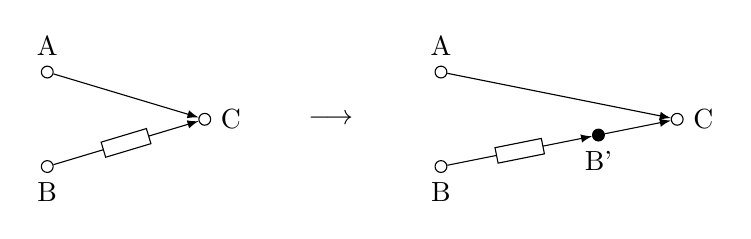
\begin{tikzpicture}[x=2cm, y=1cm]
    \tikzstyle{node0}=[circle, draw, fill=white, inner sep=0pt, minimum size=1.5mm]
    \tikzstyle{node1}=[circle, draw, fill=black, inner sep=0pt, minimum size=1.5mm]

    \node[node0, label=above:A] (A1) at (0, 0) {};
    \node[node0, label=below:B] (B1) at (0, -1.2) {};
    \node[node0, label=right:C] (C1) at (1, -0.6) {};

    \chanSync{A1}{C1}
    \chanFifoOne{B1}{C1}

    \node at (1.8, -0.6) {$\longrightarrow$};

    \node[node0, label=above:A] (A2) at (2.5, 0) {};
    \node[node0, label=below:B] (B2) at (2.5, -1.2) {};
    \node[node1, label=below:B'] (B3) at (3.5, -0.8) {};
    \node[node0, label=right:C] (C2) at (4, -0.6) {};

    \chanSync{A2}{C2}
    \chanFifoOne{B2}{B3}
    \chanSync{B3}{C2}

\end{tikzpicture}
\caption{Adding hidden node to a merger}
    \label{fig:automerger}
\end{figure}

To address this predicament, we develop an automatic merging algorithm \verb|automerger| that enables users to input the nodes only in their original forms without manually adding hidden nodes. The input includes the basic channels and the nodes to be merged. The algorithm will then search for a merger's participant channels, automatically add a hidden node with a unique name to each one (to satisfy the black box checking), and construct a new Sync channel between the hidden node and the merged node. This algorithm simplifies the process of building complex connectors involving mergers and makies the structure more intuitive and user-friendly, avoiding potential errors from manual node addition.

In addition, we upgrade the merger to a multi-merger that can merge more than two input nodes at the same time. The new merger can rearrange the data flows in a chronological order just like the original merger. The implementation of multi-merger can be found at \cite{Z3}. The \verb|automerger| algorithm works well with the multi-merger.

\subsection{Examples of test cases}
We use test cases to validate the correctness of our method, which can be found at \cite{Z3}. Here we choose three representative examples to show how the system works.

\begin{example} % 1. Basic test case
    Fig.\ref{fig:c1} contains four similar connectors, the purpose of which is to output the data flow simultaneously from two sink nodes with a delay. Graph \verb|b|, \verb|c|, and \verb|d| all complete the task perfectly by using a \textit{SyncDrain} channel to synchronize the two flows or just making the delay happens in the same \textit{FIFO1} channel. However, graph \verb|a| fails to achieve the goal since the node B and C are not constrained to be simultanuous. Hence, \verb|b|, \verb|c|, and \verb|d| are equivlent with each other, and are all refinements of \verb|a|.\par
    In our Z3 implementation, we can easily construct these four connectors and check their refinement relations. Graph \verb|a| and \verb|b| can be formalized into
    \begin{verbatim}
c1 = ['Sync A D', 'Sync D E', 'Sync D F', 'Fifo1 E B', 'Fifo1 F C']
c2 = ['Sync A D', 'Sync D E', 'Sync D F', 'Fifo1 E G', 'Fifo1 F H',
      'SyncDrain G H','Sync G B', 'Sync H C']
    \end{verbatim}
    After constructing them into the \verb|Connector| class by the function \verb|automerger|, the result aligns with what we expect: \verb|c1.isRefinementOf(c2, bound)| returns \verb|False| with a counter example, while \verb|c2.isRefinementOf(c1, bound)| returns \verb|True|. The equivalence between \verb|c2|, \verb|c3|, and \verb|c4| can also be verified in the same way.
\end{example}
\begin{figure}[htbp]
    \centering
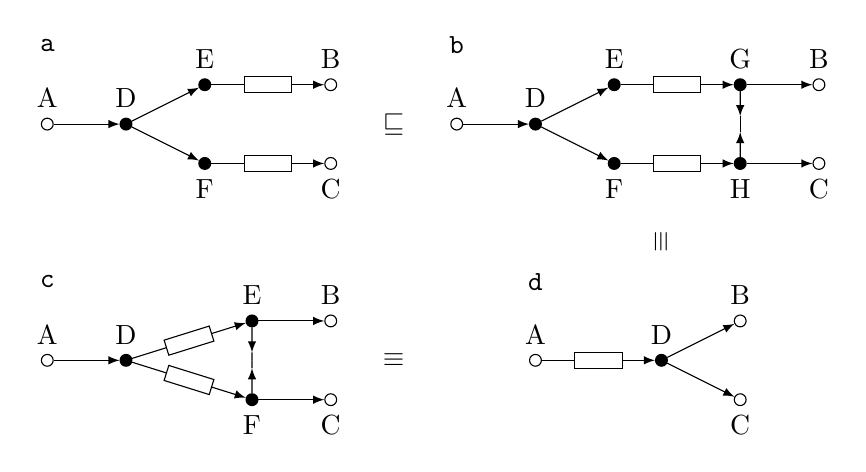
\begin{tikzpicture}[x=2cm, y=1cm]

    % connector 1
    \node[node0, label=above:A] (A1) at (0, -0.5) {};
    \node[node0, label=above:B] (B1) at (1.8, 0) {};
    \node[node0, label=below:C] (C1) at (1.8, -1) {};
    \node[node1, label=above:D] (D1) at (0.5, -0.5) {};
    \node[node1, label=above:E] (E1) at (1, 0) {};
    \node[node1, label=below:F] (F1) at (1, -1) {};

    \chanSync{A1}{D1}
    \chanSync{D1}{E1}
    \chanSync{D1}{F1}
    \chanFifoOne{E1}{B1}
    \chanFifoOne{F1}{C1}

    \node at (0, 0.5) {\verb|a|};

    \node at (2.2, -0.5) {$\sqsubseteq$};

    % connector 2
    \coordinate (off2) at (2.6, 0);
    \node[node0, label=above:A] (A2) at ($(off2) + (0, -0.5)$) {};
    \node[node0, label=above:B] (B2) at ($(off2) + (2.3, 0)$) {};
    \node[node0, label=below:C] (C2) at ($(off2) + (2.3, -1)$) {};
    \node[node1, label=above:D] (D2) at ($(off2) + (0.5, -0.5)$) {};
    \node[node1, label=above:E] (E2) at ($(off2) + (1, 0)$) {};
    \node[node1, label=below:F] (F2) at ($(off2) + (1, -1)$) {};
    \node[node1, label=above:G] (G2) at ($(off2) + (1.8, 0)$) {};
    \node[node1, label=below:H] (H2) at ($(off2) + (1.8, -1)$) {};

    \chanSync{A2}{D2}
    \chanSync{D2}{E2}
    \chanSync{D2}{F2}
    \chanFifoOne{E2}{G2}
    \chanFifoOne{F2}{H2}
    \chanSyncDrain{G2}{H2}
    \chanSync{G2}{B2}
    \chanSync{H2}{C2}

    \node at ($(off2)+(0, 0.5)$) {\verb|b|};

    \node[rotate=90] at (3.9, -2) {$\equiv$};

    % connector 3
    \coordinate (off3) at (0, -3);
    \node[node0, label=above:A] (A1) at ($(off3) + (0, -0.5)$) {};
    \node[node0, label=above:B] (B1) at ($(off3) + (1.8, 0)$) {};
    \node[node0, label=below:C] (C1) at ($(off3) + (1.8, -1)$) {};
    \node[node1, label=above:D] (D1) at ($(off3) + (0.5, -0.5)$) {};
    \node[node1, label=above:E] (E1) at ($(off3) + (1.3, 0)$) {};
    \node[node1, label=below:F] (F1) at ($(off3) + (1.3, -1)$) {};

    \chanSync{A1}{D1}
    \chanFifoOne{D1}{E1}
    \chanFifoOne{D1}{F1}
    \chanSyncDrain{E1}{F1}
    \chanSync{E1}{B1}
    \chanSync{F1}{C1}

    \node at ($(off3)+(0, 0.5)$) {\verb|c|};

    \node at (2.2, -3.5) {$\equiv$};

    % connector 4
    \coordinate (off4) at (3.1, -3);
    \node[node0, label=above:A] (A1) at ($(off4) + (0, -0.5)$) {};
    \node[node0, label=above:B] (B1) at ($(off4) + (1.3, 0)$) {};
    \node[node0, label=below:C] (C1) at ($(off4) + (1.3, -1)$) {};
    \node[node1, label=above:D] (D1) at ($(off4) + (0.8, -0.5)$) {};

    \chanFifoOne{A1}{D1}
    \chanSync{D1}{B1}
    \chanSync{D1}{C1}

    \node at ($(off4)+(0, 0.5)$) {\verb|d|};

\end{tikzpicture}
\caption{Basic test case}
    \label{fig:c1}
\end{figure}

\begin{example} % 2. Time-based test case
    The left graph in Fig.\ref{fig:c2} is called Lower Bounded FIFO1, which aims to output the data flow with a delay of at least $t$ time units. The right graph is a mutated connector of the former one, since it requires the output time to be exactly $t$ time units later than the input time. Hence in Z3 implementation, the result of \verb|isRefinementOf| between the two connectors would be both \verb|False| with counter examples.
\end{example}
\begin{figure}[htbp]
    \centering
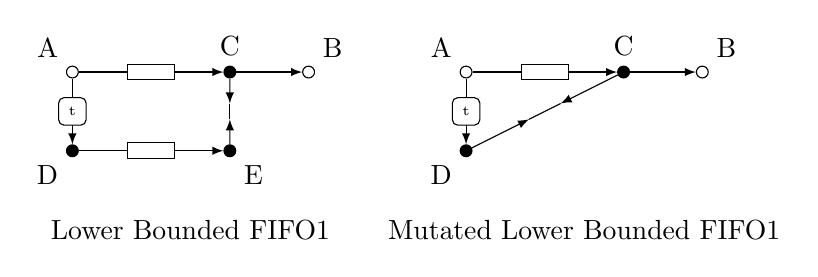
\begin{tikzpicture}[x=2cm, y=1cm]

    % connector 1
    \node[node0, label=above left:A] (A1) at (0, 0) {};
    \node[node0, label=above right:B] (B1) at (1.5, 0) {};
    \node[node1, label=above:C] (C1) at (1, 0) {};
    \node[node1, label=below left:D] (D1) at (0, -1) {};
    \node[node1, label=below right:E] (E1) at (1, -1) {};

    \chanFifoOne{A1}{C1}
    \chanTimert{A1}{D1}{t}
    \chanFifoOne{D1}{E1}
    \chanSyncDrain{C1}{E1}
    \chanSync{C1}{B1}

    \node at (0.75, -2) {Lower Bounded FIFO1};

    % connector 2
    \coordinate (off) at (2.5, 0);
    \node[node0, label=above left:A] (A2) at ($(off) + (0, 0)$) {};
    \node[node0, label=above right:B] (B2) at ($(off) + (1.5, 0)$) {};
    \node[node1, label=above:C] (C2) at ($(off) + (1, 0)$) {};
    \node[node1, label=below left:D] (D2) at ($(off) + (0, -1)$) {};

    \chanFifoOne{A2}{C2}
    \chanTimert{A2}{D2}{t}
    \chanSyncDrain{C2}{D2}
    \chanSync{C2}{B2}

    \node at ($(off)+(0.75, -2)$) {Mutated Lower Bounded FIFO1};

\end{tikzpicture}
\caption{Time-based test case}
    \label{fig:c2}
\end{figure}

\begin{example} % 3. Probability-based test case
    In the third example, we combine a timer channel and a probabilistic channel to form a complex connector and its mutation as shown in Fig.\ref{fig:c3}. The two connectors are supposed to output a random signal in $\{ 0, 1 \}$ after a delay of $t$ time units. The two connectors only differ in the time when the random signal is generated: before or after the delay. Therefore, they are equivalent, i.e., a refinement of each other. In Z3 implementation, we can verify this quivalence by verifying the \verb|True| output of the \verb|isRefinementOf| function in both directions.
\end{example}
\begin{figure}[htbp]
    \centering
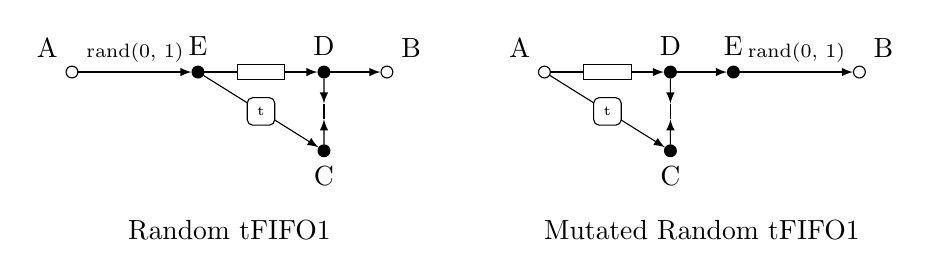
\begin{tikzpicture}[x=2cm, y=1cm]

    % connector 1
    \node[node0, label=above left:A] (A1) at (0, 0) {};
    \node[node0, label=above right:B] (B1) at (2, 0) {};
    \node[node1, label=below:C] (C1) at (1.6, -1) {};
    \node[node1, label=above:D] (D1) at (1.6, 0) {};
    \node[node1, label=above:E] (E1) at (0.8, 0) {};

    \chanRdmSync{A1}{E1}{rand(0, 1)}
    \chanFifoOne{E1}{D1}
    \chanTimert{E1}{C1}{t}
    \chanSyncDrain{C1}{D1}
    \chanSync{D1}{B1}

    \node at (1, -2) {Random tFIFO1};

    % connector 2
    \coordinate (off) at (3, 0);
    \node[node0, label=above left:A] (A1) at ($(off) + (0, 0)$) {};
    \node[node0, label=above right:B] (B1) at ($(off) + (2, 0)$) {};
    \node[node1, label=below:C] (C1) at ($(off) + (0.8, -1)$) {};
    \node[node1, label=above:D] (D1) at ($(off) + (0.8, 0)$) {};
    \node[node1, label=above:E] (E1) at ($(off) + (1.2, 0)$) {};

    \chanSync{D1}{E1}
    \chanFifoOne{A1}{D1}
    \chanTimert{A1}{C1}{t}
    \chanSyncDrain{C1}{D1}
    \chanRdmSync{E1}{B1}{rand(0, 1)}

    \node at ($(off)+(1, -2)$) {Mutated Random tFIFO1};

\end{tikzpicture}
\caption{Probability-based test case}
    \label{fig:c3}
\end{figure}

\section{Conclusion and future work}
\label{sec:conclusion}
This paper presents a unified framework for the formal modeling, refinement verification, and test case generation of Reo connectors by integrating UTP-based semantics with automated reasoning using Z3. The framework establishes a coherent foundation for reasoning about connector behavior, correctness, and test adequacy.\par
We extend the UTP design model to encompass basic, timed, and probabilistic Reo connectors. By explicitly distinguishing preconditions and postconditions, the proposed model makes input–output causality explicit and supports uniform reasoning about heterogeneous connector behaviors, including timing constraints and probabilistic effects.\par
The Z3-based realization enables automated refinement checking and fault-based test case generation. Refinement verification is reduced to constraint solving, allowing the automatic detection of invalid refinements through bounded counterexamples and alleviating the reliance on interactive theorem proving. Moreover, fault-based test cases are systematically derived from specifications and faulty implementations, facilitating the detection of common design errors such as incorrect channel types and topology mismatches.\par
To support scalable connector construction, we introduce an automerger algorithm and a multi-merger extension that automate node merging and hiding. These mechanisms reduce manual intervention and help ensure the correctness of complex connector compositions. Experimental results indicate that the framework effectively supports connector modeling, refinement and equivalence checking, and automated test case generation.\par
Future work includes extending the framework to richer quantitative constraints, improving the scalability of automated verification, and validating the approach in larger and more realistic application scenarios. Overall, this work provides a rigorous and practical basis for the formal development and validation of Reo-based coordination systems.


\nocite{*}
\bibliography{reference}

\end{document}
